\documentclass{article}
\usepackage{amsmath}
\usepackage[margin=1in]{geometry}
\usepackage{amsfonts}
\usepackage{hyperref}
\usepackage{graphicx}
\usepackage{amssymb}

\begin{document}
	
	\title{Determinant}
	\author{Andy Chong Sam}
	
	\maketitle	
	
	\section{Geometric Intuition of Determinants}
	
	\par \noindent This introduction offers a geometric intuition of the determinant in two and three dimensions. We start with the idea of a \textbf{square matrix} which is one that has an equal number of rows and columns. A 2x2 square matrix is therefore capable of holding two vectors each containing 2 components, and a 3x3 matrix can hold three vectors each containing 3 components.
	\newline
	\newline
	\begin{minipage}[c]{.45\linewidth}
		\par \noindent Let's consider a generic 2x2 matrix containing two linearly independent vectors: \{\(\vec a, \vec b\)\}.
		\newline
		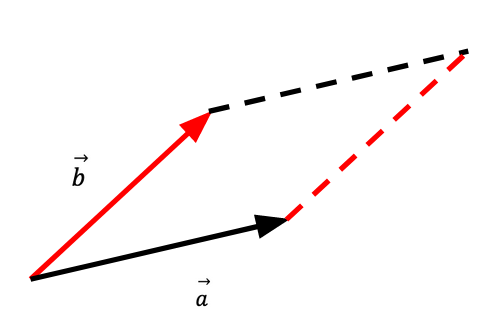
\includegraphics[width=5cm]{det-geo1.png}\newline
		\begin{center}Figure 1\end{center}
		\par \noindent The two vectors form a parallelogram. The determinant of a matrix containing \{\(\vec a, \vec b\)\} will be the area of this parallelogram.  
		\newline
		\par \noindent Given a matrix A comprised of vectors \(\vec a\) and \( \vec b\):
		\[A=
		\left(\begin{array}{@{}cc@{}}
			a_x & b_x \\ 
			a_y &  b_y \\
		\end{array}\right)
		\]
		\newline
		\par \noindent The determinant is:
		
		\begin{flalign*}
		 det(A)=a_xb_y - b_xa_y
		 \end{flalign*}
		\newline
		\par \noindent How the formula is derived will be the subject of section 2.
				
	\end{minipage}
	\hspace{0.75cm}
	\begin{minipage}[c]{.45\linewidth}
		\par \noindent  Let's consider a generic 3x3 matrix containing three linearly independent vectors: \{\(\vec a, \vec b, \vec c\)\}.
		\newline
		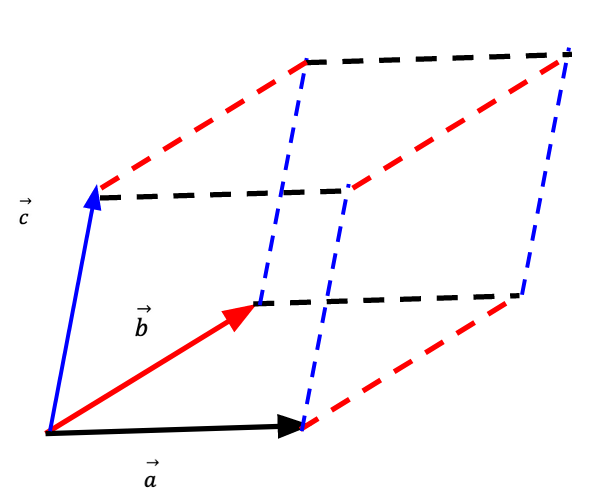
\includegraphics[width=5cm]{det-geo2.png}
		\begin{center}Figure 2\end{center}
		\par \noindent The three vectors form a parallelepiped. The determinant of a matrix containing \{\(\vec a, \vec b, \vec c\)\} when calculated will be the volume of the parallelepiped. 
		\newline
		\par\noindent Given a matrix B comprised of \(\vec a\), \(\vec b\) \(\vec c\):
		 \[B=
		 \left(\begin{array}{@{}ccc@{}}
		 	a_x & b_x & c_x \\ 
		 	a_y &  b_y & c_y \\
		 	a_z &  b_z & c_z \\
		 \end{array}\right)
		 \]
		\par \noindent The determinant is:
		\begin{flalign*}
		det(B)=(a_xb_yc_z+a_zb_xc_y + a_yb_zc_x) -(a_zb_yc_x + a_xb_zc_y + a_yb_xc_z)
		\end{flalign*}
		\par \noindent The above formula was derived using the \textbf{triple scalar product}, and will be expanded upon in section 3.
		 \(\)
	\end{minipage}
\newpage
\section{A 2x2 matrix}
\par \noindent To show that the determinant of a 2x2 matrix is the area of the parallelogram from figure 1 we can start by defining matrix A made comprised of two generic vectors. This vector along with its determinant is shown below:
\[A=
\left(\begin{array}{@{}cc@{}}
	a_x & b_x \\ 
	a_y &  b_y \\
\end{array}\right)
\therefore det(A) = a_x b_y - b_x a_y\]
\newline
\par\noindent 
	\begin{minipage}[c]{.25\linewidth}
		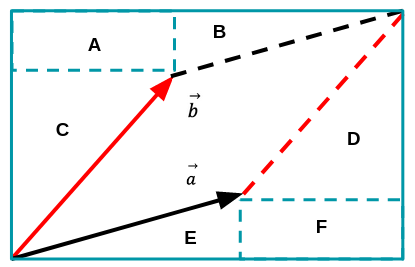
\includegraphics[width=5cm]{parallelogram2by2.png}\newline
\end{minipage}
\hspace{0.75cm}
\begin{minipage}[c]{.75\linewidth}
	\par \noindent \textbf{(Total Area)} \(= (a_x + b_x)(a_y + b_y)=a_xa_y+a_xb_y + b_xa_y+b_xb_y\)
	\par\noindent \textbf{(A \& F)} = \(b_xa_y\), \textbf{(B \& E)}=\(\frac{1}{2}a_xa_y\), \textbf{(C \& D)}=\(\frac{1}{2}b_xb_y\)
\end{minipage}
\par\noindent The area of the inscribed parallelogram can will be the Total Rectangle Area minus the sum of the named components. This result is the determinant of matrix A:
\begin{flalign*}
	a_xa_y + a_xb_y + b_xa_y + b_xb_y - 2b_xa_y - a_xa_y - b_xb_y \\
	=a_xb_y + b_xa_y - 2b_xa_y \\
	=a_xb_y - b_xa_y	
\end{flalign*}
\section{A 3x3 matrix}
\par\noindent The determinant of a 3x3 matrix is the volume of a parallelepiped. This can be conveyed through the following matrix: 
		 \[B=
\left(\begin{array}{@{}ccc@{}}
	a_x & b_x & c_x \\ 
	a_y &  b_y & c_y \\
	a_z &  b_z & c_z \\
\end{array}\right) \therefore det(B)=(a_xb_yc_z+a_zb_xc_y + a_yb_zc_x) -(a_zb_yc_x + a_xb_zc_y + a_yb_xc_z)
\]


	\begin{minipage}[c]{.25\linewidth}
	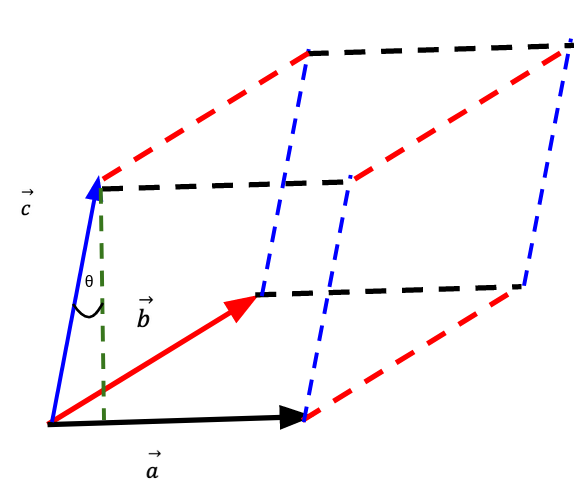
\includegraphics[width=5cm]{parallelipiped.png}\newline
\end{minipage}
\hspace{0.75cm}
\begin{minipage}[c]{.75\linewidth}
	
	\par \noindent The volume of such a figure will be its base multiplied by its height. 
	\newline
	\par \noindent The base will be the parallelogram \( || \vec a \times \vec b  ||\), and the height will be \(||\vec c||cos \theta\). We can simplify the volume \(||\vec a \times \vec b||\)  \(||c||cos \theta\) using the law of cosines to: \(  (\vec a \times \vec b)\cdot \vec c\) .
\end{minipage}
\par\noindent We can now carry out the triple scalar operation which will the determinant of matrix B:
\[  (\vec a \times \vec b)\cdot \vec c=
\left(\begin{array}{@{}c@{}}
	c_x \\ 
	c_y \\
	c_z
\end{array}\right) \cdot 
\left(\begin{array}{@{}ccc@{}}
	a_yb_z - a_zb_y & -a_xb_z + a_zb_x & a_xb_y-a_yb_x
\end{array}\right)
\]

\begin{flalign*}
	c_x(a_yb_z-a_zb_y) + c_y(-a_xb_z+a_zb_x) + c_z(a_xb_y - a_yb_x)	\\
	= a_yb_zc_x - a_zb_yc_x - a_xb_zc_y + a_zb_xc_y + a_xb_yc_z - a_yb_xc_z \\
	= (a_xb_yc_z + a_zb_xc_y + a_yb_zc_x) - (a_zb_yc_x + a_xb_zc_y + a_yb_xc_z)
\end{flalign*}
\end{document}